% Options for packages loaded elsewhere
% Options for packages loaded elsewhere
\PassOptionsToPackage{unicode}{hyperref}
\PassOptionsToPackage{hyphens}{url}
\PassOptionsToPackage{dvipsnames,svgnames,x11names}{xcolor}
%
\documentclass[
  letterpaper,
  DIV=11,
  numbers=noendperiod]{scrartcl}
\usepackage{xcolor}
\usepackage{amsmath,amssymb}
\setcounter{secnumdepth}{-\maxdimen} % remove section numbering
\usepackage{iftex}
\ifPDFTeX
  \usepackage[T1]{fontenc}
  \usepackage[utf8]{inputenc}
  \usepackage{textcomp} % provide euro and other symbols
\else % if luatex or xetex
  \usepackage{unicode-math} % this also loads fontspec
  \defaultfontfeatures{Scale=MatchLowercase}
  \defaultfontfeatures[\rmfamily]{Ligatures=TeX,Scale=1}
\fi
\usepackage{lmodern}
\ifPDFTeX\else
  % xetex/luatex font selection
\fi
% Use upquote if available, for straight quotes in verbatim environments
\IfFileExists{upquote.sty}{\usepackage{upquote}}{}
\IfFileExists{microtype.sty}{% use microtype if available
  \usepackage[]{microtype}
  \UseMicrotypeSet[protrusion]{basicmath} % disable protrusion for tt fonts
}{}
\makeatletter
\@ifundefined{KOMAClassName}{% if non-KOMA class
  \IfFileExists{parskip.sty}{%
    \usepackage{parskip}
  }{% else
    \setlength{\parindent}{0pt}
    \setlength{\parskip}{6pt plus 2pt minus 1pt}}
}{% if KOMA class
  \KOMAoptions{parskip=half}}
\makeatother
% Make \paragraph and \subparagraph free-standing
\makeatletter
\ifx\paragraph\undefined\else
  \let\oldparagraph\paragraph
  \renewcommand{\paragraph}{
    \@ifstar
      \xxxParagraphStar
      \xxxParagraphNoStar
  }
  \newcommand{\xxxParagraphStar}[1]{\oldparagraph*{#1}\mbox{}}
  \newcommand{\xxxParagraphNoStar}[1]{\oldparagraph{#1}\mbox{}}
\fi
\ifx\subparagraph\undefined\else
  \let\oldsubparagraph\subparagraph
  \renewcommand{\subparagraph}{
    \@ifstar
      \xxxSubParagraphStar
      \xxxSubParagraphNoStar
  }
  \newcommand{\xxxSubParagraphStar}[1]{\oldsubparagraph*{#1}\mbox{}}
  \newcommand{\xxxSubParagraphNoStar}[1]{\oldsubparagraph{#1}\mbox{}}
\fi
\makeatother

\usepackage{color}
\usepackage{fancyvrb}
\newcommand{\VerbBar}{|}
\newcommand{\VERB}{\Verb[commandchars=\\\{\}]}
\DefineVerbatimEnvironment{Highlighting}{Verbatim}{commandchars=\\\{\}}
% Add ',fontsize=\small' for more characters per line
\usepackage{framed}
\definecolor{shadecolor}{RGB}{241,243,245}
\newenvironment{Shaded}{\begin{snugshade}}{\end{snugshade}}
\newcommand{\AlertTok}[1]{\textcolor[rgb]{0.68,0.00,0.00}{#1}}
\newcommand{\AnnotationTok}[1]{\textcolor[rgb]{0.37,0.37,0.37}{#1}}
\newcommand{\AttributeTok}[1]{\textcolor[rgb]{0.40,0.45,0.13}{#1}}
\newcommand{\BaseNTok}[1]{\textcolor[rgb]{0.68,0.00,0.00}{#1}}
\newcommand{\BuiltInTok}[1]{\textcolor[rgb]{0.00,0.23,0.31}{#1}}
\newcommand{\CharTok}[1]{\textcolor[rgb]{0.13,0.47,0.30}{#1}}
\newcommand{\CommentTok}[1]{\textcolor[rgb]{0.37,0.37,0.37}{#1}}
\newcommand{\CommentVarTok}[1]{\textcolor[rgb]{0.37,0.37,0.37}{\textit{#1}}}
\newcommand{\ConstantTok}[1]{\textcolor[rgb]{0.56,0.35,0.01}{#1}}
\newcommand{\ControlFlowTok}[1]{\textcolor[rgb]{0.00,0.23,0.31}{\textbf{#1}}}
\newcommand{\DataTypeTok}[1]{\textcolor[rgb]{0.68,0.00,0.00}{#1}}
\newcommand{\DecValTok}[1]{\textcolor[rgb]{0.68,0.00,0.00}{#1}}
\newcommand{\DocumentationTok}[1]{\textcolor[rgb]{0.37,0.37,0.37}{\textit{#1}}}
\newcommand{\ErrorTok}[1]{\textcolor[rgb]{0.68,0.00,0.00}{#1}}
\newcommand{\ExtensionTok}[1]{\textcolor[rgb]{0.00,0.23,0.31}{#1}}
\newcommand{\FloatTok}[1]{\textcolor[rgb]{0.68,0.00,0.00}{#1}}
\newcommand{\FunctionTok}[1]{\textcolor[rgb]{0.28,0.35,0.67}{#1}}
\newcommand{\ImportTok}[1]{\textcolor[rgb]{0.00,0.46,0.62}{#1}}
\newcommand{\InformationTok}[1]{\textcolor[rgb]{0.37,0.37,0.37}{#1}}
\newcommand{\KeywordTok}[1]{\textcolor[rgb]{0.00,0.23,0.31}{\textbf{#1}}}
\newcommand{\NormalTok}[1]{\textcolor[rgb]{0.00,0.23,0.31}{#1}}
\newcommand{\OperatorTok}[1]{\textcolor[rgb]{0.37,0.37,0.37}{#1}}
\newcommand{\OtherTok}[1]{\textcolor[rgb]{0.00,0.23,0.31}{#1}}
\newcommand{\PreprocessorTok}[1]{\textcolor[rgb]{0.68,0.00,0.00}{#1}}
\newcommand{\RegionMarkerTok}[1]{\textcolor[rgb]{0.00,0.23,0.31}{#1}}
\newcommand{\SpecialCharTok}[1]{\textcolor[rgb]{0.37,0.37,0.37}{#1}}
\newcommand{\SpecialStringTok}[1]{\textcolor[rgb]{0.13,0.47,0.30}{#1}}
\newcommand{\StringTok}[1]{\textcolor[rgb]{0.13,0.47,0.30}{#1}}
\newcommand{\VariableTok}[1]{\textcolor[rgb]{0.07,0.07,0.07}{#1}}
\newcommand{\VerbatimStringTok}[1]{\textcolor[rgb]{0.13,0.47,0.30}{#1}}
\newcommand{\WarningTok}[1]{\textcolor[rgb]{0.37,0.37,0.37}{\textit{#1}}}

\usepackage{longtable,booktabs,array}
\usepackage{calc} % for calculating minipage widths
% Correct order of tables after \paragraph or \subparagraph
\usepackage{etoolbox}
\makeatletter
\patchcmd\longtable{\par}{\if@noskipsec\mbox{}\fi\par}{}{}
\makeatother
% Allow footnotes in longtable head/foot
\IfFileExists{footnotehyper.sty}{\usepackage{footnotehyper}}{\usepackage{footnote}}
\makesavenoteenv{longtable}
\usepackage{graphicx}
\makeatletter
\newsavebox\pandoc@box
\newcommand*\pandocbounded[1]{% scales image to fit in text height/width
  \sbox\pandoc@box{#1}%
  \Gscale@div\@tempa{\textheight}{\dimexpr\ht\pandoc@box+\dp\pandoc@box\relax}%
  \Gscale@div\@tempb{\linewidth}{\wd\pandoc@box}%
  \ifdim\@tempb\p@<\@tempa\p@\let\@tempa\@tempb\fi% select the smaller of both
  \ifdim\@tempa\p@<\p@\scalebox{\@tempa}{\usebox\pandoc@box}%
  \else\usebox{\pandoc@box}%
  \fi%
}
% Set default figure placement to htbp
\def\fps@figure{htbp}
\makeatother





\setlength{\emergencystretch}{3em} % prevent overfull lines

\providecommand{\tightlist}{%
  \setlength{\itemsep}{0pt}\setlength{\parskip}{0pt}}



 


\KOMAoption{captions}{tableheading}
\makeatletter
\@ifpackageloaded{caption}{}{\usepackage{caption}}
\AtBeginDocument{%
\ifdefined\contentsname
  \renewcommand*\contentsname{Table of contents}
\else
  \newcommand\contentsname{Table of contents}
\fi
\ifdefined\listfigurename
  \renewcommand*\listfigurename{List of Figures}
\else
  \newcommand\listfigurename{List of Figures}
\fi
\ifdefined\listtablename
  \renewcommand*\listtablename{List of Tables}
\else
  \newcommand\listtablename{List of Tables}
\fi
\ifdefined\figurename
  \renewcommand*\figurename{Figure}
\else
  \newcommand\figurename{Figure}
\fi
\ifdefined\tablename
  \renewcommand*\tablename{Table}
\else
  \newcommand\tablename{Table}
\fi
}
\@ifpackageloaded{float}{}{\usepackage{float}}
\floatstyle{ruled}
\@ifundefined{c@chapter}{\newfloat{codelisting}{h}{lop}}{\newfloat{codelisting}{h}{lop}[chapter]}
\floatname{codelisting}{Listing}
\newcommand*\listoflistings{\listof{codelisting}{List of Listings}}
\makeatother
\makeatletter
\makeatother
\makeatletter
\@ifpackageloaded{caption}{}{\usepackage{caption}}
\@ifpackageloaded{subcaption}{}{\usepackage{subcaption}}
\makeatother
\usepackage{bookmark}
\IfFileExists{xurl.sty}{\usepackage{xurl}}{} % add URL line breaks if available
\urlstyle{same}
\hypersetup{
  pdftitle={Quantifying the Texas blackout of 2021},
  pdfauthor={Leela Dixit},
  colorlinks=true,
  linkcolor={blue},
  filecolor={Maroon},
  citecolor={Blue},
  urlcolor={Blue},
  pdfcreator={LaTeX via pandoc}}


\title{Quantifying the Texas blackout of 2021}
\author{Leela Dixit}
\date{2025-11-10}
\begin{document}
\maketitle


In early 2021, Texas experienced three extreme weather events resulting
in a major power grid blackout. This blackout caused inhospitable
conditions for many homes in Texas, with shortages of food, water, and
heat. In this project, we will quantify the amount of homes in Houston
that were affected by the outage, and investigate whether these impacts
disproportionately affected certain census groups such as income.

\begin{Shaded}
\begin{Highlighting}[]
\CommentTok{\# load packages}
\FunctionTok{library}\NormalTok{(tidyverse)}
\FunctionTok{library}\NormalTok{(dplyr)}
\FunctionTok{library}\NormalTok{(here)}
\FunctionTok{library}\NormalTok{(sf)}
\FunctionTok{library}\NormalTok{(stars)}
\FunctionTok{library}\NormalTok{(terra)}
\FunctionTok{library}\NormalTok{(raster)}
\FunctionTok{library}\NormalTok{(tmap)}
\end{Highlighting}
\end{Shaded}

\begin{Shaded}
\begin{Highlighting}[]
\CommentTok{\# read in data}
\NormalTok{query\_road }\OtherTok{\textless{}{-}} \StringTok{"SELECT * FROM gis\_osm\_roads\_free\_1 WHERE fclass=\textquotesingle{}motorway\textquotesingle{}"}
\NormalTok{roads }\OtherTok{\textless{}{-}} \FunctionTok{st\_read}\NormalTok{(}\FunctionTok{here}\NormalTok{(}\StringTok{"data"}\NormalTok{, }\StringTok{"gis\_osm\_roads\_free\_1.gpkg"}\NormalTok{), }\AttributeTok{query =}\NormalTok{ query\_road)}

\NormalTok{query\_houses }\OtherTok{\textless{}{-}} \StringTok{"SELECT * FROM gis\_osm\_buildings\_a\_free\_1 WHERE (type IS NULL AND name IS NULL) OR type in (\textquotesingle{}residential\textquotesingle{}, \textquotesingle{}apartments\textquotesingle{}, \textquotesingle{}house\textquotesingle{}, \textquotesingle{}static\_caravan\textquotesingle{}, \textquotesingle{}detached\textquotesingle{})"}
\NormalTok{houses }\OtherTok{\textless{}{-}} \FunctionTok{st\_read}\NormalTok{(}\FunctionTok{here}\NormalTok{(}\StringTok{"data"}\NormalTok{, }\StringTok{"gis\_osm\_buildings\_a\_free\_1.gpkg"}\NormalTok{), }\AttributeTok{query =}\NormalTok{ query\_houses)}

\FunctionTok{st\_layers}\NormalTok{(}\FunctionTok{here}\NormalTok{(}\StringTok{"data"}\NormalTok{, }\StringTok{"ACS\_2019\_5YR\_TRACT\_48\_TEXAS.gdb"}\NormalTok{))}
\NormalTok{socioeconomic\_geoid }\OtherTok{\textless{}{-}} \FunctionTok{st\_read}\NormalTok{(}\FunctionTok{here}\NormalTok{(}\StringTok{"data"}\NormalTok{, }\StringTok{"ACS\_2019\_5YR\_TRACT\_48\_TEXAS.gdb"}\NormalTok{), }\AttributeTok{layer =} \StringTok{"ACS\_2019\_5YR\_TRACT\_48\_TEXAS"}\NormalTok{)}
\NormalTok{socioeconomic }\OtherTok{\textless{}{-}} \FunctionTok{st\_read}\NormalTok{(}\FunctionTok{here}\NormalTok{(}\StringTok{"data"}\NormalTok{, }\StringTok{"ACS\_2019\_5YR\_TRACT\_48\_TEXAS.gdb"}\NormalTok{), }\AttributeTok{layer =} \StringTok{"X19\_INCOME"}\NormalTok{)}

\NormalTok{light5\_207 }\OtherTok{\textless{}{-}} \FunctionTok{read\_stars}\NormalTok{(}\FunctionTok{here}\NormalTok{(}\StringTok{"data"}\NormalTok{, }\StringTok{"VNP46A1"}\NormalTok{, }\StringTok{"VNP46A1.A2021038.h08v05.001.2021039064328.tif"}\NormalTok{))}
\NormalTok{light6\_207}\OtherTok{\textless{}{-}} \FunctionTok{read\_stars}\NormalTok{(}\FunctionTok{here}\NormalTok{(}\StringTok{"data"}\NormalTok{, }\StringTok{"VNP46A1"}\NormalTok{, }\StringTok{"VNP46A1.A2021038.h08v06.001.2021039064329.tif"}\NormalTok{))}
\NormalTok{light5\_216 }\OtherTok{\textless{}{-}} \FunctionTok{read\_stars}\NormalTok{(}\FunctionTok{here}\NormalTok{(}\StringTok{"data"}\NormalTok{, }\StringTok{"VNP46A1"}\NormalTok{, }\StringTok{"VNP46A1.A2021047.h08v05.001.2021048091106.tif"}\NormalTok{))}
\NormalTok{light6\_216 }\OtherTok{\textless{}{-}} \FunctionTok{read\_stars}\NormalTok{(}\FunctionTok{here}\NormalTok{(}\StringTok{"data"}\NormalTok{, }\StringTok{"VNP46A1"}\NormalTok{, }\StringTok{"VNP46A1.A2021047.h08v06.001.2021048091105.tif"}\NormalTok{))}
\end{Highlighting}
\end{Shaded}

\section{Step 1: Find locations that experienced a blackout by creating
a
mask}\label{step-1-find-locations-that-experienced-a-blackout-by-creating-a-mask}

Join the light data and find the change between dates

\begin{Shaded}
\begin{Highlighting}[]
\CommentTok{\# join shapefiles of each tile for each day}
\NormalTok{light\_207 }\OtherTok{\textless{}{-}} \FunctionTok{st\_mosaic}\NormalTok{(light5\_207, light6\_207)}
\NormalTok{light\_216 }\OtherTok{\textless{}{-}} \FunctionTok{st\_mosaic}\NormalTok{(light5\_216, light6\_216)}

\CommentTok{\# find the change in light intensity before and after the storm}
\NormalTok{light\_change }\OtherTok{\textless{}{-}}\NormalTok{ light\_207 }\SpecialCharTok{{-}}\NormalTok{ light\_216}
\end{Highlighting}
\end{Shaded}

Visualize light intensity in Houston before and after the storm

\begin{Shaded}
\begin{Highlighting}[]
\CommentTok{\# define bbox of Houston area}
\NormalTok{bbox\_light }\OtherTok{\textless{}{-}} \FunctionTok{st\_bbox}\NormalTok{(}\FunctionTok{c}\NormalTok{(}\AttributeTok{xmin =} \SpecialCharTok{{-}}\FloatTok{96.5}\NormalTok{, }\AttributeTok{ymin =} \DecValTok{29}\NormalTok{, }\AttributeTok{xmax =} \SpecialCharTok{{-}}\FloatTok{94.5}\NormalTok{, }\AttributeTok{ymax =} \FloatTok{30.5}\NormalTok{), }\AttributeTok{crs =} \FunctionTok{st\_crs}\NormalTok{(light\_207))}
\CommentTok{\# transform bbox into sf object}
\NormalTok{bbox\_light }\OtherTok{\textless{}{-}} \FunctionTok{st\_as\_sfc}\NormalTok{(bbox\_light)}
\CommentTok{\# double check crs match before cropping}
\FunctionTok{st\_crs}\NormalTok{(bbox\_light) }\SpecialCharTok{==} \FunctionTok{st\_crs}\NormalTok{(light\_207)}
\end{Highlighting}
\end{Shaded}

\begin{verbatim}
[1] TRUE
\end{verbatim}

\begin{Shaded}
\begin{Highlighting}[]
\CommentTok{\# crop light intensities for each day to just Houston area}
\NormalTok{cropped\_light\_207 }\OtherTok{\textless{}{-}} \FunctionTok{st\_crop}\NormalTok{(light\_207, bbox\_light)}
\NormalTok{cropped\_light\_216 }\OtherTok{\textless{}{-}} \FunctionTok{st\_crop}\NormalTok{(light\_216, bbox\_light)}
\end{Highlighting}
\end{Shaded}

\begin{Shaded}
\begin{Highlighting}[]
\CommentTok{\# map each day to see the light change}
\NormalTok{map\_207 }\OtherTok{\textless{}{-}} \FunctionTok{tm\_shape}\NormalTok{(cropped\_light\_207) }\SpecialCharTok{+}
  \FunctionTok{tm\_raster}\NormalTok{(}\AttributeTok{palette =} \StringTok{"Greys"}\NormalTok{,}
            \AttributeTok{breaks =} \FunctionTok{c}\NormalTok{(}\DecValTok{0}\NormalTok{, }\DecValTok{100}\NormalTok{, }\DecValTok{200}\NormalTok{, }\DecValTok{500}\NormalTok{, }\DecValTok{800}\NormalTok{, }\DecValTok{1000}\NormalTok{, }\ConstantTok{Inf}\NormalTok{),}
            \AttributeTok{title =} \StringTok{"Night light intensity }
\StringTok{(200 nW cm{-}2sr{-}1)"}\NormalTok{) }\SpecialCharTok{+}
  \FunctionTok{tm\_title}\NormalTok{(}\StringTok{"Light Intensity Pre{-}Storm"}\NormalTok{) }\SpecialCharTok{+}
  \FunctionTok{tm\_compass}\NormalTok{() }\SpecialCharTok{+}
  \FunctionTok{tm\_scalebar}\NormalTok{()}
\CommentTok{\# }
\NormalTok{map\_216 }\OtherTok{\textless{}{-}} \FunctionTok{tm\_shape}\NormalTok{(cropped\_light\_216) }\SpecialCharTok{+}
  \FunctionTok{tm\_raster}\NormalTok{(}\AttributeTok{palette =} \StringTok{"Greys"}\NormalTok{,}
            \AttributeTok{breaks =} \FunctionTok{c}\NormalTok{(}\DecValTok{0}\NormalTok{, }\DecValTok{100}\NormalTok{, }\DecValTok{200}\NormalTok{, }\DecValTok{500}\NormalTok{, }\DecValTok{800}\NormalTok{, }\DecValTok{1000}\NormalTok{, }\ConstantTok{Inf}\NormalTok{),}
            \AttributeTok{title =} \StringTok{"Night light intensity }
\StringTok{(200 nW cm{-}2sr{-}1)"}\NormalTok{) }\SpecialCharTok{+}
  \FunctionTok{tm\_title}\NormalTok{(}\StringTok{"Light Intensity Post{-}Storm"}\NormalTok{) }\SpecialCharTok{+}
  \FunctionTok{tm\_compass}\NormalTok{() }\SpecialCharTok{+}
  \FunctionTok{tm\_scalebar}\NormalTok{()}

\FunctionTok{tmap\_arrange}\NormalTok{(map\_207, map\_216, }\AttributeTok{nrow =} \DecValTok{1}\NormalTok{)}
\end{Highlighting}
\end{Shaded}

\pandocbounded{\includegraphics[keepaspectratio]{texas_blackout_files/figure-pdf/unnamed-chunk-6-1.pdf}}

Create mask to define which areas experienced a blackout

\begin{Shaded}
\begin{Highlighting}[]
\CommentTok{\# transform from stars to raster object}
\NormalTok{light\_change }\OtherTok{\textless{}{-}} \FunctionTok{rast}\NormalTok{(light\_change)}

\CommentTok{\# define matrix for values greater than 200 nw}
\NormalTok{rcl }\OtherTok{\textless{}{-}} \FunctionTok{matrix}\NormalTok{(}\FunctionTok{c}\NormalTok{(}\SpecialCharTok{{-}}\ConstantTok{Inf}\NormalTok{, }\DecValTok{200}\NormalTok{, }\ConstantTok{NA}\NormalTok{,}
                \DecValTok{200}\NormalTok{, }\ConstantTok{Inf}\NormalTok{, }\ConstantTok{TRUE}\NormalTok{),}
              \AttributeTok{ncol =} \DecValTok{3}\NormalTok{, }\AttributeTok{byrow =} \ConstantTok{TRUE}\NormalTok{)}

\CommentTok{\# apply mask for values \textgreater{} 200 nW}
\NormalTok{reclass\_light }\OtherTok{\textless{}{-}} \FunctionTok{classify}\NormalTok{(light\_change, }\AttributeTok{rcl =}\NormalTok{ rcl)}
\NormalTok{reclass\_light}
\end{Highlighting}
\end{Shaded}

Transform light difference to a vector

\begin{Shaded}
\begin{Highlighting}[]
\CommentTok{\# check crs of masked light dataframe}
\FunctionTok{st\_crs}\NormalTok{(reclass\_light)}\SpecialCharTok{$}\NormalTok{epsg}
\end{Highlighting}
\end{Shaded}

\begin{verbatim}
[1] 4326
\end{verbatim}

\begin{Shaded}
\begin{Highlighting}[]
\CommentTok{\# transform from rast to sf object to vectorize}
\NormalTok{light\_change\_vector }\OtherTok{\textless{}{-}}\NormalTok{ reclass\_light }\SpecialCharTok{\%\textgreater{}\%} 
  \FunctionTok{st\_as\_stars}\NormalTok{() }\SpecialCharTok{\%\textgreater{}\%} 
  \FunctionTok{st\_as\_sf}\NormalTok{() }\SpecialCharTok{\%\textgreater{}\%} 
  \FunctionTok{st\_make\_valid}\NormalTok{()}

\CommentTok{\# check type of vectorized data frame}
\FunctionTok{class}\NormalTok{(light\_change\_vector)}
\end{Highlighting}
\end{Shaded}

\begin{verbatim}
[1] "sf"         "data.frame"
\end{verbatim}

crop (spatially subset) the blackout mask to the Houston area

\begin{Shaded}
\begin{Highlighting}[]
\CommentTok{\# redefine bbox for Houston area}
\NormalTok{bbox\_crop }\OtherTok{\textless{}{-}} \FunctionTok{st\_bbox}\NormalTok{(}\FunctionTok{c}\NormalTok{(}\AttributeTok{xmin =} \SpecialCharTok{{-}}\FloatTok{96.5}\NormalTok{, }\AttributeTok{ymin =} \DecValTok{29}\NormalTok{, }\AttributeTok{xmax =} \SpecialCharTok{{-}}\FloatTok{94.5}\NormalTok{, }\AttributeTok{ymax =} \FloatTok{30.5}\NormalTok{), }\AttributeTok{crs =} \FunctionTok{st\_crs}\NormalTok{(light\_change\_vector))}
\CommentTok{\# transform bbox to sf object}
\NormalTok{bbox\_crop }\OtherTok{\textless{}{-}} \FunctionTok{st\_as\_sfc}\NormalTok{(bbox\_crop)}
\CommentTok{\# double check class}
\FunctionTok{class}\NormalTok{(bbox\_crop)}
\end{Highlighting}
\end{Shaded}

\begin{verbatim}
[1] "sfc_POLYGON" "sfc"        
\end{verbatim}

\begin{Shaded}
\begin{Highlighting}[]
\CommentTok{\# double check crs match}
\FunctionTok{st\_crs}\NormalTok{(bbox\_crop) }\SpecialCharTok{==} \FunctionTok{st\_crs}\NormalTok{(light\_change\_vector)}
\end{Highlighting}
\end{Shaded}

\begin{verbatim}
[1] TRUE
\end{verbatim}

\begin{Shaded}
\begin{Highlighting}[]
\CommentTok{\# crop vectorized light object to just Houston area}
\NormalTok{cropped\_light\_diff }\OtherTok{\textless{}{-}} \FunctionTok{st\_crop}\NormalTok{(light\_change\_vector, bbox\_crop)}
\end{Highlighting}
\end{Shaded}

Reproject the crs of the light change data

\begin{Shaded}
\begin{Highlighting}[]
\CommentTok{\# reproject vectorized data to NAD83 crs}
\NormalTok{cropped\_light\_diff }\OtherTok{\textless{}{-}} \FunctionTok{st\_transform}\NormalTok{(cropped\_light\_diff, }\AttributeTok{crs =} \StringTok{"epsg:3083"}\NormalTok{)}
\FunctionTok{st\_crs}\NormalTok{(cropped\_light\_diff)}\SpecialCharTok{$}\NormalTok{epsg}
\end{Highlighting}
\end{Shaded}

\begin{verbatim}
[1] 3083
\end{verbatim}

Plot the areas of Houston that experienced a blackout

\begin{Shaded}
\begin{Highlighting}[]
\CommentTok{\# plot Houston that experienced a blackout}
\FunctionTok{tm\_shape}\NormalTok{(cropped\_light\_diff) }\SpecialCharTok{+}
  \FunctionTok{tm\_fill}\NormalTok{(}\AttributeTok{fill =} \StringTok{"black"}\NormalTok{) }\SpecialCharTok{+}
  \FunctionTok{tm\_basemap}\NormalTok{(}\StringTok{"CartoDB.PositronNoLabels"}\NormalTok{) }\SpecialCharTok{+}
  \FunctionTok{tm\_title}\NormalTok{(}\StringTok{"Areas of Houston that experienced a blackout"}\NormalTok{) }\SpecialCharTok{+}
  \FunctionTok{tm\_compass}\NormalTok{(}\AttributeTok{position =} \FunctionTok{tm\_pos\_in}\NormalTok{(}\StringTok{"left"}\NormalTok{, }\StringTok{"bottom"}\NormalTok{)) }\SpecialCharTok{+}
  \FunctionTok{tm\_scalebar}\NormalTok{(}\AttributeTok{position =} \FunctionTok{tm\_pos\_in}\NormalTok{(}\StringTok{"left"}\NormalTok{, }\StringTok{"bottom"}\NormalTok{))}
\end{Highlighting}
\end{Shaded}

\begin{verbatim}
[plot mode] fit legend/component: Some legend items or map compoments do not
fit well, and are therefore rescaled.
i Set the tmap option `component.autoscale = FALSE` to disable rescaling.
\end{verbatim}

\pandocbounded{\includegraphics[keepaspectratio]{texas_blackout_files/figure-pdf/unnamed-chunk-11-1.pdf}}

\section{Step 2: Exclude highways from
analysis}\label{step-2-exclude-highways-from-analysis}

Find areas around highways to exclude from the analysis

\begin{Shaded}
\begin{Highlighting}[]
\CommentTok{\# check units of roads and transform}
\FunctionTok{st\_crs}\NormalTok{(roads, }\AttributeTok{parameters =} \ConstantTok{TRUE}\NormalTok{)}\SpecialCharTok{$}\NormalTok{units\_gdal }\CommentTok{\# its in degree units}
\end{Highlighting}
\end{Shaded}

\begin{verbatim}
[1] "degree"
\end{verbatim}

\begin{Shaded}
\begin{Highlighting}[]
\NormalTok{roads }\OtherTok{\textless{}{-}} \FunctionTok{st\_transform}\NormalTok{(roads, }\FunctionTok{st\_crs}\NormalTok{(cropped\_light\_diff))}
\FunctionTok{st\_crs}\NormalTok{(roads, }\AttributeTok{parameters =} \ConstantTok{TRUE}\NormalTok{)}\SpecialCharTok{$}\NormalTok{units\_gdal }\CommentTok{\# now it is in metre}
\end{Highlighting}
\end{Shaded}

\begin{verbatim}
[1] "metre"
\end{verbatim}

\begin{Shaded}
\begin{Highlighting}[]
\CommentTok{\# create buffer of 200 m around roadways}
\NormalTok{roads\_200 }\OtherTok{\textless{}{-}} \FunctionTok{st\_buffer}\NormalTok{(roads, }\AttributeTok{dist =} \DecValTok{200}\NormalTok{)}
\CommentTok{\# join with roads to treat as one road 200m large}
\NormalTok{roads\_200 }\OtherTok{\textless{}{-}} \FunctionTok{st\_union}\NormalTok{(roads\_200)}
\CommentTok{\# plot quickly to check it worked}
\NormalTok{map\_road }\OtherTok{\textless{}{-}} \FunctionTok{tm\_shape}\NormalTok{(roads) }\SpecialCharTok{+}
  \FunctionTok{tm\_lines}\NormalTok{() }\SpecialCharTok{+}
  \FunctionTok{tm\_title}\NormalTok{(}\StringTok{"Before buffer"}\NormalTok{)}
\NormalTok{map\_road\_200 }\OtherTok{\textless{}{-}} \FunctionTok{tm\_shape}\NormalTok{(roads\_200) }\SpecialCharTok{+}
  \FunctionTok{tm\_lines}\NormalTok{() }\SpecialCharTok{+}
  \FunctionTok{tm\_title}\NormalTok{(}\StringTok{"After buffer"}\NormalTok{)}
\FunctionTok{tmap\_arrange}\NormalTok{(map\_road, map\_road\_200, }\AttributeTok{nrow =} \DecValTok{1}\NormalTok{)}
\end{Highlighting}
\end{Shaded}

\pandocbounded{\includegraphics[keepaspectratio]{texas_blackout_files/figure-pdf/unnamed-chunk-12-1.pdf}}

find areas that experienced blackouts that are further than 200m from a
highway

\begin{Shaded}
\begin{Highlighting}[]
\CommentTok{\# check CRS match}
\FunctionTok{st\_crs}\NormalTok{(roads\_200)}\SpecialCharTok{$}\NormalTok{epsg }\SpecialCharTok{==} \FunctionTok{st\_crs}\NormalTok{(cropped\_light\_diff)}\SpecialCharTok{$}\NormalTok{epsg}
\end{Highlighting}
\end{Shaded}

\begin{verbatim}
[1] TRUE
\end{verbatim}

\begin{Shaded}
\begin{Highlighting}[]
\CommentTok{\# find areas of Houston that experienced blackout that are not near roads}
\NormalTok{light\_road\_clip }\OtherTok{\textless{}{-}} \FunctionTok{st\_difference}\NormalTok{(cropped\_light\_diff, roads\_200)}

\CommentTok{\# plot to see where they overlapped}
\FunctionTok{tm\_shape}\NormalTok{(light\_road\_clip) }\SpecialCharTok{+}
  \FunctionTok{tm\_polygons}\NormalTok{() }\SpecialCharTok{+}
\FunctionTok{tm\_shape}\NormalTok{(roads\_200) }\SpecialCharTok{+}
  \FunctionTok{tm\_lines}\NormalTok{(}\AttributeTok{col\_alpha =} \FloatTok{0.5}\NormalTok{, }
           \AttributeTok{col =} \StringTok{"red"}\NormalTok{) }\SpecialCharTok{+}
  \FunctionTok{tm\_title}\NormalTok{(}\StringTok{"Homes that experienced a blackout in Houston, Texas"}\NormalTok{) }\SpecialCharTok{+}
  \FunctionTok{tm\_title}\NormalTok{(}\StringTok{"200m away from highways"}\NormalTok{, }\AttributeTok{size =} \FloatTok{0.9}\NormalTok{) }\SpecialCharTok{+}
  \FunctionTok{tm\_add\_legend}\NormalTok{(}\AttributeTok{type =} \StringTok{"lines"}\NormalTok{, }
                \AttributeTok{labels =} \FunctionTok{c}\NormalTok{(}\StringTok{"200m highway buffer"}\NormalTok{),}
                \AttributeTok{col =} \FunctionTok{c}\NormalTok{(}\StringTok{"red"}\NormalTok{)) }\SpecialCharTok{+}
  \FunctionTok{tm\_layout}\NormalTok{(}\AttributeTok{legend.position =} \FunctionTok{c}\NormalTok{(}\StringTok{"left"}\NormalTok{, }\StringTok{"bottom"}\NormalTok{))}
\end{Highlighting}
\end{Shaded}

\pandocbounded{\includegraphics[keepaspectratio]{texas_blackout_files/figure-pdf/unnamed-chunk-13-1.pdf}}

\section{Step 3: Identify homes that experienced blackouts by combining
the locations of homes and
blackouts}\label{step-3-identify-homes-that-experienced-blackouts-by-combining-the-locations-of-homes-and-blackouts}

Find homes that experienced a blackout

\begin{Shaded}
\begin{Highlighting}[]
\CommentTok{\# check crs match}
\FunctionTok{st\_crs}\NormalTok{(light\_road\_clip) }\SpecialCharTok{==} \FunctionTok{st\_crs}\NormalTok{(houses) }
\end{Highlighting}
\end{Shaded}

\begin{verbatim}
[1] FALSE
\end{verbatim}

\begin{Shaded}
\begin{Highlighting}[]
\CommentTok{\# transform crs to match }
\NormalTok{houses }\OtherTok{\textless{}{-}} \FunctionTok{st\_transform}\NormalTok{(houses, }\FunctionTok{st\_crs}\NormalTok{(light\_road\_clip))}
\CommentTok{\# check crs match}
\FunctionTok{st\_crs}\NormalTok{(light\_road\_clip) }\SpecialCharTok{==} \FunctionTok{st\_crs}\NormalTok{(houses) }
\end{Highlighting}
\end{Shaded}

\begin{verbatim}
[1] TRUE
\end{verbatim}

\begin{Shaded}
\begin{Highlighting}[]
\CommentTok{\# find homes that experienced a blackout}
\NormalTok{homes\_blackout }\OtherTok{\textless{}{-}} \FunctionTok{st\_intersection}\NormalTok{(light\_road\_clip, houses)}
\end{Highlighting}
\end{Shaded}

Visualize homes that experienced a blackout

\begin{Shaded}
\begin{Highlighting}[]
\CommentTok{\# plot homes in Houston that experienced a blackout}
\FunctionTok{tm\_shape}\NormalTok{(homes\_blackout) }\SpecialCharTok{+}
  \FunctionTok{tm\_polygons}\NormalTok{() }\SpecialCharTok{+}
  \FunctionTok{tm\_basemap}\NormalTok{(}\StringTok{"CartoDB.PositronNoLabels"}\NormalTok{) }\SpecialCharTok{+}
  \FunctionTok{tm\_title}\NormalTok{(}\StringTok{"Homes that experienced a blackout in Houston, Texas"}\NormalTok{)}
\end{Highlighting}
\end{Shaded}

\begin{verbatim}
[plot mode] fit legend/component: Some legend items or map compoments do not
fit well, and are therefore rescaled.
i Set the tmap option `component.autoscale = FALSE` to disable rescaling.
\end{verbatim}

\pandocbounded{\includegraphics[keepaspectratio]{texas_blackout_files/figure-pdf/unnamed-chunk-15-1.pdf}}

\begin{Shaded}
\begin{Highlighting}[]
  \FunctionTok{tm\_compass}\NormalTok{(}\AttributeTok{position =} \FunctionTok{tm\_pos\_in}\NormalTok{(}\StringTok{"left"}\NormalTok{, }\StringTok{"bottom"}\NormalTok{)) }\SpecialCharTok{+}
  \FunctionTok{tm\_scalebar}\NormalTok{(}\AttributeTok{position =} \FunctionTok{tm\_pos\_in}\NormalTok{(}\StringTok{"left"}\NormalTok{, }\StringTok{"bottom"}\NormalTok{))}
\end{Highlighting}
\end{Shaded}

\begin{verbatim}
[nothing to show] no data layers defined
\end{verbatim}

Find the number of homes that experienced a blackout

\begin{Shaded}
\begin{Highlighting}[]
\CommentTok{\# find number of homes that experienced a blackout}
\FunctionTok{nrow}\NormalTok{(homes\_blackout)}
\end{Highlighting}
\end{Shaded}

\begin{verbatim}
[1] 168874
\end{verbatim}

\section{Step 4: Identify the census tracts likely impacted by
blackout}\label{step-4-identify-the-census-tracts-likely-impacted-by-blackout}

Prepare socioeconomic data for joining

\begin{Shaded}
\begin{Highlighting}[]
\CommentTok{\# check crs of socioeconomic data}
\FunctionTok{st\_crs}\NormalTok{(socioeconomic\_geoid)}\SpecialCharTok{$}\NormalTok{epsg}
\end{Highlighting}
\end{Shaded}

\begin{verbatim}
[1] 4269
\end{verbatim}

\begin{Shaded}
\begin{Highlighting}[]
\CommentTok{\# transform to match NAD83}
\NormalTok{socioeconomic\_geoid }\OtherTok{\textless{}{-}} \FunctionTok{st\_transform}\NormalTok{(socioeconomic\_geoid, }
                                    \AttributeTok{crs =} \FunctionTok{st\_crs}\NormalTok{(homes\_blackout))}
\CommentTok{\# rename GEOID column to prep for joining}
\NormalTok{socioeconomic }\OtherTok{\textless{}{-}}\NormalTok{ socioeconomic }\SpecialCharTok{\%\textgreater{}\%} 
  \FunctionTok{rename}\NormalTok{(}\StringTok{"GEOID\_Data"} \OtherTok{=} \StringTok{"GEOID"}\NormalTok{)}
\end{Highlighting}
\end{Shaded}

Join the spatial data with the socioeconomic data

\begin{Shaded}
\begin{Highlighting}[]
\CommentTok{\# join shapefile with socioeconomic data}
\NormalTok{socioeconomic\_join }\OtherTok{\textless{}{-}} \FunctionTok{left\_join}\NormalTok{(socioeconomic\_geoid, socioeconomic,}
                                \AttributeTok{by =} \StringTok{"GEOID\_Data"}\NormalTok{)}
\CommentTok{\# transform to sf object}
\NormalTok{socioeconomic\_join }\OtherTok{\textless{}{-}} \FunctionTok{st\_as\_sf}\NormalTok{(socioeconomic\_join)}
\CommentTok{\# check the column we want was populated with data}
\NormalTok{socioeconomic\_join}\SpecialCharTok{$}\NormalTok{B19013e1}

\CommentTok{\# select for only the columns we want}
\NormalTok{socioeconomic\_join }\OtherTok{\textless{}{-}}\NormalTok{ socioeconomic\_join[, }\FunctionTok{c}\NormalTok{(}\StringTok{"TRACTCE"}\NormalTok{, }\StringTok{"GEOID\_Data"}\NormalTok{, }\StringTok{"B19013e1"}\NormalTok{)]}
\end{Highlighting}
\end{Shaded}

Find homes that did and did not experience a blackout

\begin{Shaded}
\begin{Highlighting}[]
\NormalTok{homes\_blackout\_TF }\OtherTok{\textless{}{-}}\NormalTok{ houses }\SpecialCharTok{\%\textgreater{}\%} 
  \FunctionTok{mutate}\NormalTok{(}\AttributeTok{blackout =}\NormalTok{ osm\_id }\SpecialCharTok{\%in\%}\NormalTok{ homes\_blackout}\SpecialCharTok{$}\NormalTok{osm\_id)}

\CommentTok{\# join socioeconomic data to homes that experienced a blackout}
\NormalTok{socioeconomic\_homes }\OtherTok{\textless{}{-}} \FunctionTok{st\_intersection}\NormalTok{(homes\_blackout\_TF, socioeconomic\_join)}

\CommentTok{\# socioeconomic\_blackout\_TF \textless{}{-} st\_intersection(light\_road\_clip, socioeconomic\_join)}
\end{Highlighting}
\end{Shaded}

map of the census tracts in Houston that lost power

\begin{Shaded}
\begin{Highlighting}[]
\CommentTok{\# filter census tracts that did and did not experience blackouts into different data frames}
\NormalTok{socioeconomic\_homes\_blackout }\OtherTok{\textless{}{-}}\NormalTok{ socioeconomic\_homes }\SpecialCharTok{\%\textgreater{}\%} 
  \FunctionTok{filter}\NormalTok{(blackout }\SpecialCharTok{==} \StringTok{"TRUE"}\NormalTok{)}

\NormalTok{socioeconomic\_homes\_no\_blackout }\OtherTok{\textless{}{-}}\NormalTok{ socioeconomic\_homes }\SpecialCharTok{\%\textgreater{}\%} 
  \FunctionTok{filter}\NormalTok{(blackout }\SpecialCharTok{==} \StringTok{"FALSE"}\NormalTok{)}

\CommentTok{\# map each separately}
\NormalTok{map\_blackout }\OtherTok{\textless{}{-}} \FunctionTok{tm\_shape}\NormalTok{(socioeconomic\_homes\_blackout) }\SpecialCharTok{+}
  \FunctionTok{tm\_polygons}\NormalTok{(}\AttributeTok{col =} \StringTok{"B19013e1"}\NormalTok{) }\SpecialCharTok{+}
  \FunctionTok{tm\_basemap}\NormalTok{(}\StringTok{"CartoDB.PositronNoLabels"}\NormalTok{) }\SpecialCharTok{+}
  \FunctionTok{tm\_title}\NormalTok{(}\StringTok{"Cencus tracts that lost power"}\NormalTok{) }\SpecialCharTok{+}
  \FunctionTok{tm\_layout}\NormalTok{(}\AttributeTok{legend.show =} \ConstantTok{FALSE}\NormalTok{) }\SpecialCharTok{+}
  \FunctionTok{tm\_compass}\NormalTok{(}\AttributeTok{position =} \FunctionTok{tm\_pos\_in}\NormalTok{(}\StringTok{"left"}\NormalTok{, }\StringTok{"bottom"}\NormalTok{)) }\SpecialCharTok{+}
  \FunctionTok{tm\_scalebar}\NormalTok{(}\AttributeTok{position =} \FunctionTok{tm\_pos\_in}\NormalTok{(}\StringTok{"left"}\NormalTok{, }\StringTok{"bottom"}\NormalTok{))}

\NormalTok{map\_no\_blackout }\OtherTok{\textless{}{-}} \FunctionTok{tm\_shape}\NormalTok{(socioeconomic\_homes\_no\_blackout) }\SpecialCharTok{+}
  \FunctionTok{tm\_fill}\NormalTok{(}\AttributeTok{col =} \StringTok{"B19013e1"}\NormalTok{) }\SpecialCharTok{+}
  \FunctionTok{tm\_basemap}\NormalTok{(}\StringTok{"CartoDB.PositronNoLabels"}\NormalTok{) }\SpecialCharTok{+}
  \FunctionTok{tm\_title}\NormalTok{(}\StringTok{"Census tracts that did not lose power"}\NormalTok{) }\SpecialCharTok{+}
  \FunctionTok{tm\_layout}\NormalTok{(}\AttributeTok{legend.show =} \ConstantTok{FALSE}\NormalTok{) }\SpecialCharTok{+}
  \FunctionTok{tm\_compass}\NormalTok{(}\AttributeTok{position =} \FunctionTok{tm\_pos\_in}\NormalTok{(}\StringTok{"left"}\NormalTok{, }\StringTok{"bottom"}\NormalTok{)) }\SpecialCharTok{+}
  \FunctionTok{tm\_scalebar}\NormalTok{(}\AttributeTok{position =} \FunctionTok{tm\_pos\_in}\NormalTok{(}\StringTok{"left"}\NormalTok{, }\StringTok{"bottom"}\NormalTok{))}

\NormalTok{map\_blackout\_legend }\OtherTok{\textless{}{-}} \FunctionTok{tm\_shape}\NormalTok{(socioeconomic\_homes\_blackout) }\SpecialCharTok{+}
  \FunctionTok{tm\_fill}\NormalTok{(}\AttributeTok{fill =} \StringTok{"B19013e1"}\NormalTok{) }\SpecialCharTok{+}
  \FunctionTok{tm\_layout}\NormalTok{(}\AttributeTok{legend.only =} \ConstantTok{TRUE}\NormalTok{)}

\FunctionTok{tmap\_arrange}\NormalTok{(map\_blackout, map\_no\_blackout, map\_blackout\_legend, }\AttributeTok{nrow =} \DecValTok{1}\NormalTok{)}
\end{Highlighting}
\end{Shaded}

\begin{verbatim}
[plot mode] fit legend/component: Some legend items or map compoments do not
fit well, and are therefore rescaled.
i Set the tmap option `component.autoscale = FALSE` to disable rescaling.
[plot mode] fit legend/component: Some legend items or map compoments do not
fit well, and are therefore rescaled.
i Set the tmap option `component.autoscale = FALSE` to disable rescaling.
\end{verbatim}

\pandocbounded{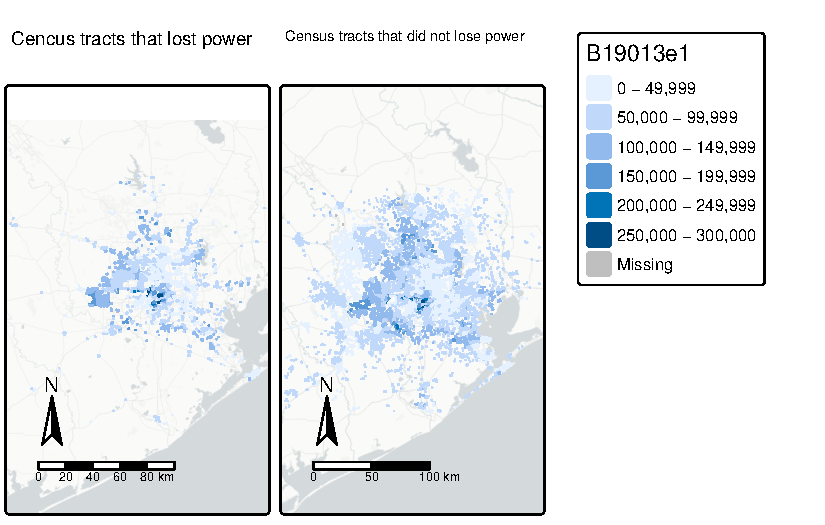
\includegraphics[keepaspectratio]{texas_blackout_files/figure-pdf/unnamed-chunk-20-1.pdf}}

Compare the distributions of median household income for census tracts
that did and did not experience blackouts

\begin{Shaded}
\begin{Highlighting}[]
\CommentTok{\# plot median household income by blackout or no blackout}
\FunctionTok{ggplot}\NormalTok{(socioeconomic\_homes, }\FunctionTok{aes}\NormalTok{(}\AttributeTok{x =}\NormalTok{ B19013e1, }\AttributeTok{fill =}\NormalTok{ blackout)) }\SpecialCharTok{+}
  \FunctionTok{geom\_histogram}\NormalTok{(}\AttributeTok{position =} \StringTok{"identity"}\NormalTok{) }\SpecialCharTok{+}
  \FunctionTok{labs}\NormalTok{(}\AttributeTok{title =} \StringTok{"Median Household Income by Blackout Experienced"}\NormalTok{,}
       \AttributeTok{x =} \StringTok{"Median household income"}\NormalTok{,}
       \AttributeTok{y =} \StringTok{"Count"}\NormalTok{) }\SpecialCharTok{+}
  \FunctionTok{theme\_classic}\NormalTok{()}
\end{Highlighting}
\end{Shaded}

\pandocbounded{\includegraphics[keepaspectratio]{texas_blackout_files/figure-pdf/unnamed-chunk-21-1.pdf}}

\begin{Shaded}
\begin{Highlighting}[]
\FunctionTok{ggplot}\NormalTok{(socioeconomic\_homes, }\FunctionTok{aes}\NormalTok{(}\AttributeTok{x =}\NormalTok{ B19013e1, }\AttributeTok{fill =}\NormalTok{ blackout)) }\SpecialCharTok{+}
  \FunctionTok{geom\_boxplot}\NormalTok{()}
\end{Highlighting}
\end{Shaded}

\pandocbounded{\includegraphics[keepaspectratio]{texas_blackout_files/figure-pdf/unnamed-chunk-21-2.pdf}}

Step 5: Conclusions - a brief reflection (approx. 100 words) summarizing
your results and discussing any limitations to this study




\end{document}
